
% \greg{TODO : interp of ConvSSM (and other models) : do we find some circuits structure similar to those found in the brain ? e.g. parallel after discharge, diverging/converging pathways, reverberating, ... ?}

\greg{TODO : references}

\paragraph{Abstract Neural Circuits.}
Neural computation in the brain is organized around circuits: structured assemblies of neurons whose collective dynamics implement specific transformations of information. Rather than isolated units or uniform layers, cortical processing emerges from patterned connectivity, where the nature of the computation is largely determined by how neurons are connected across space and time. In this work, we adopt a deliberately abstract notion of neural circuits, intended to bridge biological and artificial systems without committing to anatomical realism or specific implementation details.
%
At this level of abstraction, a neural circuit is characterized not by the biophysical properties of individual neurons, but by the organization of its connections and the resulting dynamical behavior. This perspective allows a unified treatment of biological circuits and artificial neural networks, viewing both as instances of structured dynamical systems.

\begin{definition}[Circuit]
A circuit is defined by a directed graph $(V, E)$ along with a set of dynamical equations governing the evolution of each unit $v \in V$ state over time. The dependencies between these equations are determined by the graph structure, while the specific form of the equations can vary widely.

Let $V$ be the set of units (neurons) in the circuit, and let $E \subseteq V \times V$ be the set of directed connections between them. Each connection $(u,v) \in E$ has an associated weight $w_{uv} \in \R$. The state of the circuit at time $t$ is given by a vector $h(t) \in \R^{|V|}$, where $h_v(t)$ is the activity of unit $v$ at time $t$. The evolution of the circuit's state can either be expressed in continuous time through differential equations:
\begin{equation}
\label{eq:neural_circuit:continuous}
\frac{\partial h}{\partial t}(t) = F(h(t))
\end{equation}
or in discrete time:
\begin{equation}
\label{eq:neural_circuit:discrete}
h_{t+1} = \overline{F}(h_t)
\end{equation}
where $F$ and $\overline{F}$ are functions that define the dynamics of the circuit.
\end{definition}

\begin{thomas}
\textbf{Framing suggestion.} This definition is correct but feels graph-theoretic rather than dynamical-systems. The graph $(V,E)$ and weights $w_{uv}$ are introduced but then $F$ is left completely general---so the graph structure is formally redundant until you specialize to the linear case two paragraphs later. Consider reframing around the state equation directly: start from $h'(t) = F(h(t), x(t))$ and let the connectivity \emph{emerge} as a structural property of $F$, i.e., a connection $j \to i$ exists iff $\partial F_i / \partial h_j \not\equiv 0$. This way the graph is derived from the dynamics rather than bolted on. Benefits: (1) connects directly to the SSM linearization in Part~II ($F$ linear $\Rightarrow$ $h' = Ah + Bx$, and the sparsity of $A$ \emph{is} the graph); (2) makes the stability analysis natural (eigenvalues of the Jacobian $\partial F / \partial h$); (3) lands better for the ICLR audience, who think in RNNs and state equations. You can still introduce the graph perspective when you get to the connectivity taxonomy (feedforward/feedback/lateral, circulant, block-sparse)---that's where it genuinely helps.
\end{thomas}

\begin{wrapfigure}{r}{0.3\textwidth}
    \centering
    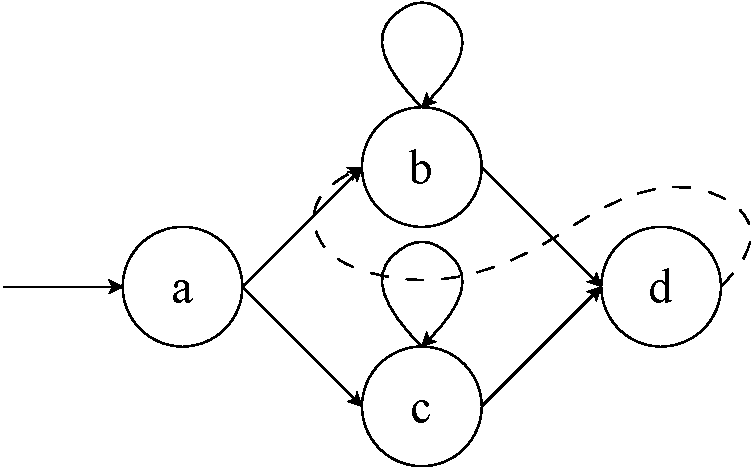
\includegraphics[width=1.0\linewidth]{figures/circuit_example.pdf}
    \caption{Example of circuit.}
    \label{fig:circuit_example}
\end{wrapfigure}

\paragraph{Input and Output Nodes.}
To prevent this system's dynamic to depend only on its initial state, we can introduce the notion of input nodes, which inject external signal into the circuit, conditioning its internal dynamics. Input nodes differ from other units in that their activity is determined externally, rather than by the circuit's internal dynamics : $h_{\mathrm{input}}(t) = x(t)$ where $x(t)$ is the external input signal at time $t$. Some nodes might also play the role of output nodes, whose activity is read out by other circuits or systems. These output nodes are readily modelled by selecting a subset of $V$. Input and output nodes provide an interface with other circuits or sensory/motor systems. \Cref{fig:circuit_example} provides an example of basic circuit with an input node $a$, recurrent connections on nodes $b$ and $c$ and feedback connections from $d$ to $b$. Its set of differential equations is given below~:

\begin{align*}
    &h_a(t) = x(t),&h_b'(t) &= (h_a + h_b + h_d)(t),\\
    &h_c'(t) = (h_a + h_c)(t),&h_d'(t) &= (h_b + h_c)(t)
\end{align*}

\begin{thomas}
Note: these equations are all linear with unit weights ($w_{uv}=1$) and no nonlinearity. Node $a$ is the input (driven externally). Node $b$ receives input from $a$ (feedforward), from itself (self-recurrence), and from $d$ (feedback). Node $c$ receives from $a$ and itself. Node $d$ receives from $b$ and $c$ (feedforward from a lower ``layer''). This matches the graph in Figure~\ref{fig:circuit_example}. The system is a coupled linear ODE: $\mathbf{h}' = W\mathbf{h} + \mathbf{b}x(t)$, where $W$ encodes the connectivity.
\end{thomas}

\paragraph{Circuit Scales.}
At the finest level, a circuit's units may correspond to individual neurons, while at coarser levels they may represent populations of neurons, other circuits, or entire brain regions. Fine-grained circuits may be embedded within larger-scale networks, with interactions occurring across multiple spatial and temporal scales. They often exhibit block-structured connectivity patterns, both in biological and artificial systems, where blocks are commonly referred to as layers due to their hierarchical arrangement with respect to information flow from input units. These blocks can be \emph{contracted} into single nodes, whose edges with other blocks represent the connectivity pattern between the units of the two blocks.

\paragraph{Connectivity structure.}
The most common models both for biological and artificial neural systems define $F$ as a linear transformation followed by a pointwise nonlinearity, as in \Cref{eq:neural_circuit:continuous_linear,eq:neural_circuit:discrete_linear}. On the biological side, this choice is motivated by the observation that neurons integrate their inputs linearly through synaptic potentials before generating spikes via a nonlinear activation function. On the artificial side, this formulation has proven effective for learning complex functions through gradient-based optimization and GPU acceleration.
\begin{align}
\label{eq:neural_circuit:continuous_linear}
\frac{ \partial h}{\partial t}(t) &= \sigma\left(W h(t) + b \right)\\
\label{eq:neural_circuit:discrete_linear}
h_{t+1} &= \sigma\left(\overline{W} h_t + \overline{b}\right)
\end{align}

\begin{thomas}
These are the ``standard neural network'' equations. In continuous time, $h'(t) = \sigma(Wh(t)+b)$ is a nonlinear ODE---much harder to analyze and simulate than the linear version. The nonlinearity $\sigma$ is applied pointwise (e.g., ReLU, sigmoid). Note: this places the nonlinearity \emph{outside} the linear transformation, matching the biological interpretation of synaptic integration (linear) followed by spike generation (nonlinear). The later SSM framework (\Cref{sec:ConvSSM_definition}) will drop $\sigma$ inside the recurrence to make it linear and parallelizable, applying nonlinearity only between layers.
\end{thomas}

where $W \in \R^{|V| \times |V|}$ is the weight matrix with $W_{uv} = w_{uv}$ if $(u,v) \in E$ and $0$ otherwise, $b \in \R^{|V|}$ is a bias vector, and $\sigma$ is a pointwise nonlinearity. However, other types of interactions are possible, such as multiplicative (or divisive) interactions (used in the KV circuits of attention layers, or [TODO: biological example]), which can then generate gating mechanisms (GRU, [TODO: biological example]), etc.

However, modeling $W$ is often impractical as $|V|$ grows large, due to the quadratic growth in the number of parameters. Therefore, structured connectivity patterns are often imposed to reduce the number of parameters. Incorporating prior knowledge about the task or data can guide the choice of connectivity structure, improving learning efficiency and generalization by providing inductive biases aligned with the underlying problem.

The most wide spread type of structure is that of block sparsity provided by a layered structure, where connections are only allowed between specific layers. Let $L_0, ..., L_n$ provide the layered structure, with layers sorted from input to output, and neurons ordered based on their layer membership.
Directed bloc connectivity can be separated into \emph{feedforward}, \emph{feedback} and \emph{recurrent} connections. When units from layer $L_i$ project onto units in layer $L_j$, we refer to \emph{feedforward} connections when $i < j$, \emph{feedback} when $i > j$ and \emph{recurrent} when $i=j$ (see \Cref{fig:connection_type}). The latter are also commonly referred to as \emph{lateral} or \emph{horizontal} connections based on author and context. In the present work, we distinguish between \emph{self-} recurrent connections to and from the same unit, and \emph{lateral} connections between arbitrary units of the same layer in order to avoid confusion between the special and general cases.

\begin{figure}[h]
    \centering
    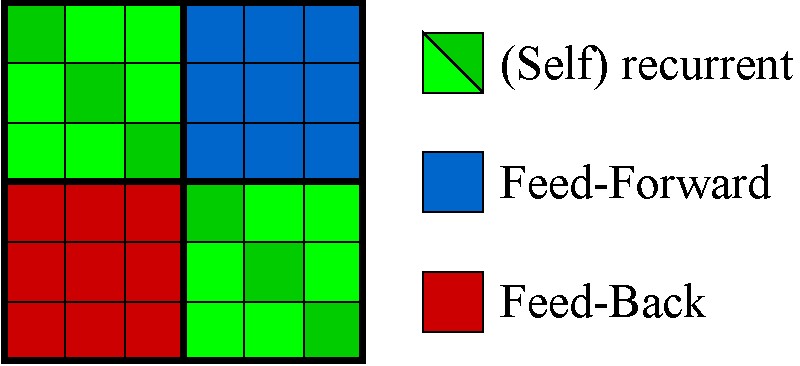
\includegraphics[width=0.5\linewidth]{figures/connection_type (1).pdf}
    \caption{Illustration of adjacency matrix, with connections colored by type. Nodes are grouped by layer and sorted from input to output.}
    \label{fig:connection_type}
\end{figure}

We can further refine the connectivity by imposing structure on blocks of the adjacency matrix. The most common type of such structure is that of \emph{local} connections, where connections are spatially constrained to a spatial neighborhood. This translates to diagonal sparsity in the corresponding block (\Cref{fig:horizontal_vs_circulant} left). This structure is famously salient in the visual cortex and in convolutional neural networks (CNN). Another common structure is that of repeating circuits \citep{TODO:visualroutine}, translating in \emph{circulant} connectivity (\Cref{fig:horizontal_vs_circulant} right). Such structure naturally models repeating microcircuits and implies translational equivariance. It can also be found in the visual cortex and in CNNs where it is typically combined with \emph{locality} leading to very efficient operationalization through convolution kernels.

\begin{figure}[h]
    \centering
    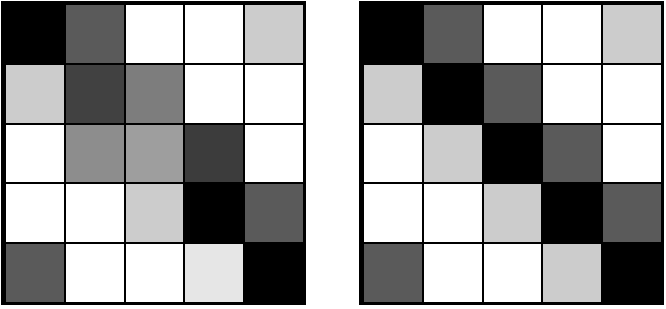
\includegraphics[width=0.5\linewidth]{figures/horizontal_vs_circulant.pdf}
    \caption{\textbf{Left~:} illustration of a block containing horizontal connections. \textbf{Right~:} a circulant matrix, imposing translational invariance on top of locality.}
    \label{fig:horizontal_vs_circulant}
\end{figure}

% TODO : make sure to mention these implementation issues but not in this section !
% \emph{Feedforward} connections are the most common, support the propagation of sensory information along processing hierarchies, as exemplified by early sensory pathways. \emph{Feedback} connections are also crucial, allowing higher layers to modulate lower layers, implementing top-down modulation and predictive signals in biological systems, though they are less frequently used in artificial systems due to training difficulties and sequentiality issues making them impractical for hardware acceleration. The same goes for \emph{recurrent} connections, which are also less common in artificial systems for the same reasons, despite being essential to model temporal dependencies and maintain internal state, integrating information over time. They implement dynamical behaviors such as attractor states, persistent activity and working memory.

% TODO : mention this extreme sparsity but not in this section. Also mention that it is true in FF and REC but not in FB, where longer range connections are possible
% Another example is that of \emph{horizontal} connections, e.g. in vision processing, where spatial locality is imposed by limiting connections to local neighborhoods, making $W$'s support a sparse number of diagonals (up to a permutation of the neuron ordering). This allows visual systems with a huge number of neurons to have a manageable number edges. With additional translational invariance constraints, $W$ becomes circulant, leading to convolutional structures. This is illustrated in \Cref{fig:horizontal_vs_circulant}. The efficiency of such local constraints is empirically verified, on the artificial side, by the success of convolutional neural networks, as well as convolutional recurrent networks such as hGRU \citep{TODO:hGRU}. On the biological side, horizontal connections in the visual cortex are known to implement functions such as [TODO:biological horizontal connections]. They are made relevant through the phenomena of \emph{retinotopy}, or the orderly mapping of the visual world from the retina onto the visual cortex, with spatial neighborhoods in the visual field maping to spatial neighborhoods in the visual cortex. They provide contextual integration, competition and naturally structured representations.

\greg{TODO : delete the paragraph below. Put it, along with other practical commentaries, in a dedicated section.}
\paragraph{Flesh vs. Silicon Circuits.}
Circuits play a fundamental role in both biological and artificial neural systems. In the brain, specialised circuits underlie sensory processing, motor control, memory, and cognition. Examples of biological circuits include cortical microcircuits with recurrent and lateral connections, thalamocortical loops, and hippocampal networks involved in memory. [TODO: expand on biological circuits examples]. \Cref{fig:CNN_vs_cortex} illustrates the whole circuit of the visual cortex, while \Cref{fig:biological_sub_circuit} shows [TODO : a sub circuit implementing some known function].

\begin{figure}[h]
    \centering
    \begin{subfigure}{0.2\linewidth}
        \centering
        
\includegraphics[width=\linewidth]{figures/placeholder.pdf}
        \caption{TODO}
        \label{fig:biological_circuit_example}
    \end{subfigure}
    \hfill
    \begin{subfigure}{0.2\linewidth}
        \centering
        
\includegraphics[width=\linewidth]{figures/placeholder.pdf}
        \caption{TODO}
        \label{fig:artificial_circuit_example}
    \end{subfigure}
    \hfill
    \begin{subfigure}{0.2\linewidth}
        \centering
        
\includegraphics[width=\linewidth]{figures/placeholder.pdf}
        \caption{TODO}
        \label{fig:adjacency_equivalence}
    \end{subfigure}
    \caption{TODO}
    \label{fig:CNN_vs_cortex}
\end{figure}

In artificial neural networks, circuit-like architectures such as recurrent networks, convolutional neural networks (CNN) with lateral connections, and attention mechanisms enable complex temporal and spatial processing capabilities. Architectures are often designed to mimic biological circuit connectivity patterns and functions. The term also refers to specific features of some architectures, such as the Key-Query (KQ) and Output-Value (OV) circuits in transformer attention mechanisms.
Artificial settings also allow for easier studies of fine grained circuits and sub-circuits implementing specific functions. Examples of such sub-circuits are known to implement specific computations such as working memory in recurrent architectures, edge detection or higher level feature extraction in visual systems. In language models, circuits have been identified that implement specific linguistic functions such as syntactic processing, as well as higher level semantic functions. \Cref{fig:CNN_vs_cortex} illustrates the full structure of a CNN mimicking the visual cortex, while \Cref{fig:artificial_sub_circuit} shows an example of sub-circuit in GPT2 implementing indirect object identification, along with each component's role in this circuit. \greg{TODO : citations !}

\begin{figure}[h]
    \centering
    \begin{subfigure}{0.2\linewidth}
        \centering
        
\includegraphics[width=\linewidth]{figures/placeholder.pdf}
        \caption{TODO}
        \label{fig:biological_sub_circuit}
    \end{subfigure}
    \hfill
    \begin{subfigure}{0.2\linewidth}
        \centering
        
\includegraphics[width=\linewidth]{figures/placeholder.pdf}
        \caption{TODO}
        \label{fig:artificial_sub_circuit}
    \end{subfigure}
    \caption{TODO}
    \label{fig:sub_circuit_illustration}
\end{figure}

